\subsection{Scaling}\label{subsec:scaling}
Scaling is implemented for the gage level measurements since baseline levels vary drastically across locations because they are determined in a fairly arbitrary manner.
For instance, Station 02160991,  located in the Broad River near Jenkinsville in South Carolina, has an average gage height of more than 200 feet \hl{(61 meters)}, while the Waccamaw River, for example, has a much lower average gage height.

To account for the disparity, we use $ y_{ij} -\tilde{y}_{i\cdot}$ as the response variable, where $ y_{ij}$ is the original gage height  for location $i$ on the $ j$th day, and $\tilde{y}_{i\cdot}$ is the median of location $i$ over 10 years.
Figure~\ref{fig:ts_plot_gage} is a time series plot of the gage heights of five randomly selected locations after scaling.

\begin{figure}[htbp]
 \begin{center}
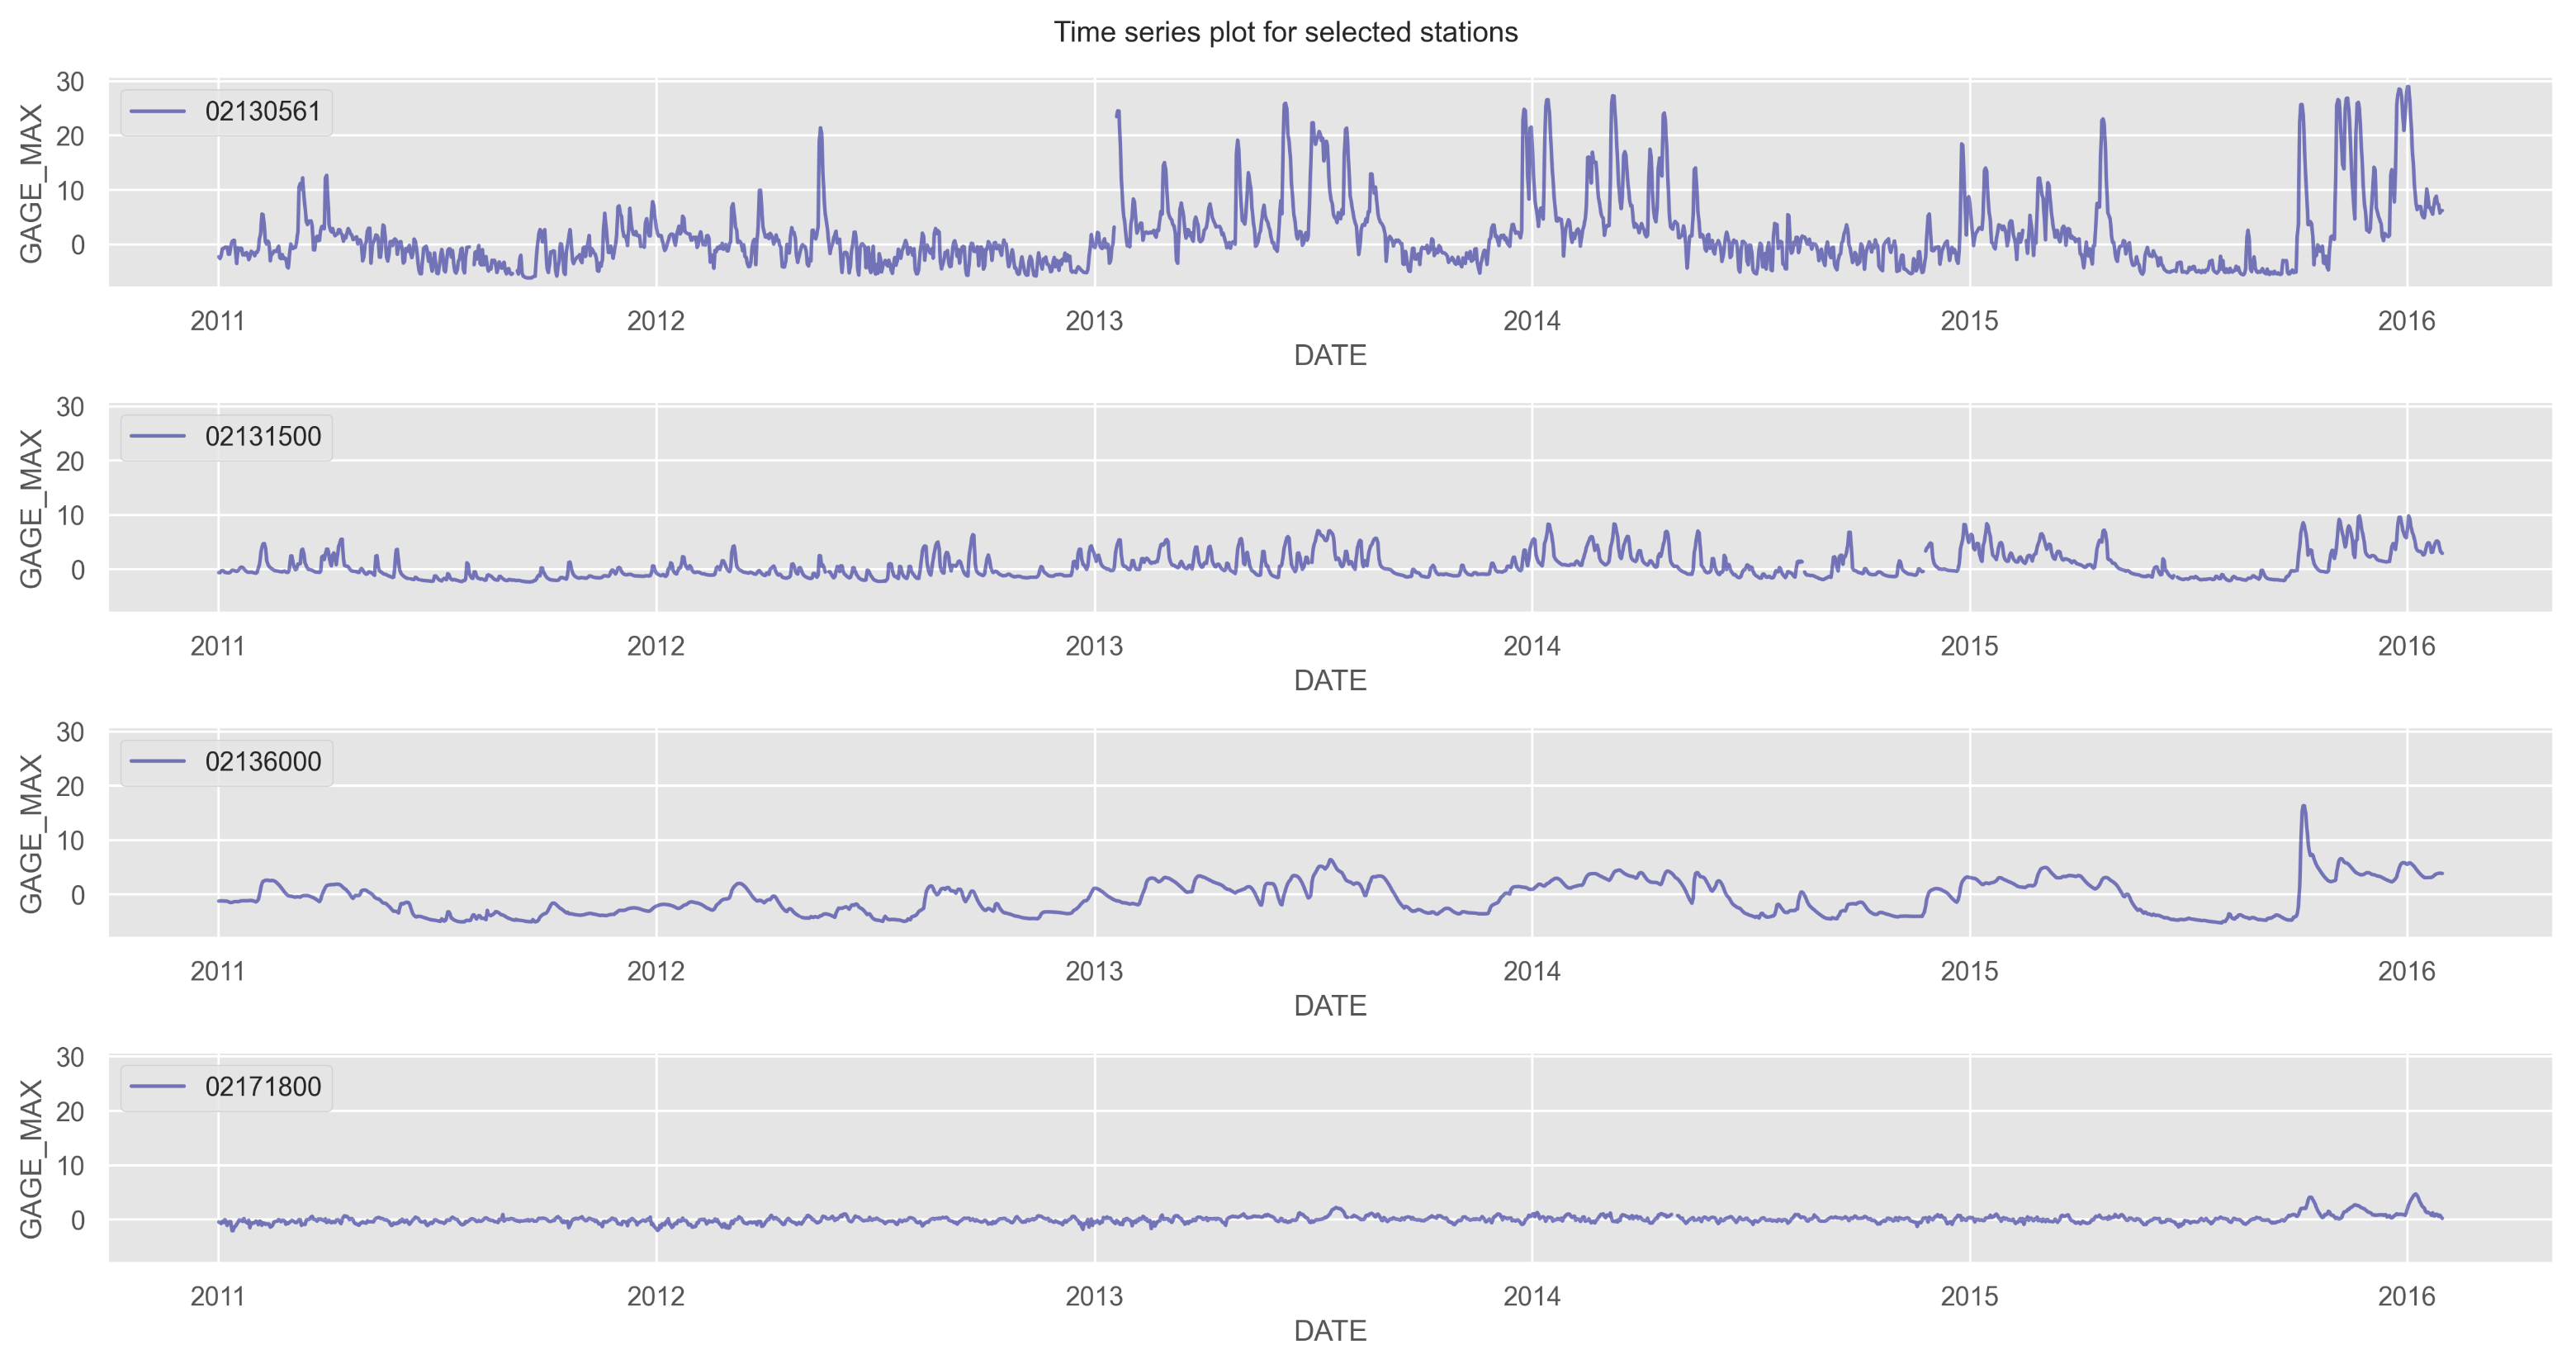
\includegraphics[width=1\textwidth]{../images/time_series_plots_four_stations.png}
\caption{\hl{Time series plot for four randomly selected gaging stations after the median level has been subtracted off.}}
\label{fig:ts_plot_gage}
 \end{center}
\end{figure}

\subsection{Autoregressive Terms}\label{subsec:autoregressive-terms}
Autoregressive terms were considered for inclusion in the model with the covariates such as precipitation since it might conceivably take days for precipitation to cause a significant rise in the gage level.
The optimal number of terms were determined by inspecting the ACF and PACF of the residuals, along with a comparison of mean squared errors with models with more or fewer autoregressive terms.
A first-order autoregressive term was used in the finalized model, and a detailed discussion can be found in Section~\ref{sec:diag}.

\subsection{Result}\label{subsec:reported_result}
We now present the model fitting results using the CAR model described in Section~\ref{sec:model}; recall that we specify a t error distribution to account for the heavy-tailed behavior of the random errors, as explained further in Section~\ref{sec:diag}.
We sample four chains from the posterior distribution of $\boldsymbol{\beta}$, $\tau$ and $\rho$, and 95\% credible intervals are reported as follows.
For each chain we ran 50,000 iterations, and the burn-in period was set to 5,000.
We experimented with both the Metropolis sampler and the No-U-Turn sampler and found that both yield similar credible intervals.
 Winter is used as the baseline season, and a positive estimate for summer, for example, indicates a rise in the predicted gage height compared to winter.
 Additionally, we found that elevation  was not significantly related to the gage level and thus is not included in the final model. \\

As seen from Table~\ref{parameter estimate}, precipitation has a significant effect on the flood level, and a rise of one inch \hl{(2.54 centimeter)} precipitation leads to an 0.25 inch \hl{(0.64 centimeter)} increase in the gage measurements on average during the winter season.
Among all the seasons, only summer stands out with a statistically significant effect on the gage height.
A positive estimate indicates a 0.041 inch \hl{(0.10 centimeter)} higher predicted gage level for a summer day than a winter day, assuming the days had no precipitation.
More importantly, the interaction between the summer season and precipitation has a positive estimate, which indicates that the effect of rainfall on gage levels are different across seasons.
Specifically, during  summer,  rainfall contributes to a larger rise (0.03 inch, or  \hl{0.08 centimeter} more) in the predicted gage level.
In other words, a stronger association between precipitation and flooding can be observed during summer compared to other times of the year.
 Lastly, a positive estimate of $ \alpha$ suggests that the locations within the same watershed are positively associated, while a positive estimate of $ \rho$ indicates that an autoregressive effect is present between different days: For example, a large gage height at a particular location is very likely to be followed by a large gage height measurement the next day at that location.
This implies that the relationships between model parameters and covariates can reflect physical mechanisms of runoff generation at a watershed scale.
When the model parameters and the covariates have a stochastic pattern/behavior (in time), the model structure reflects more complex nonlinear temporal patterns and relationships between a response variable and the covariates.
In this context, spatio-temporal variability of the interface needs to be deduced by meta-data such as effects of water abstraction scheduling, dams' construction and operation, etc.\ as recently concluded by Serinaldi and Kilsby (2015), and Samadi and Meadows (2017).

\begin{table*}[htbp]
\caption{Parameter estimates of CAR model.}
\centering
\begin{tabular}{|c|l|l|l|}
\hline
Parameter &  Variable &   Point Estimate & 95\%  Credible Interval\\ \hline
$ \beta_0$ & Intercept  &-0.0376  & (-0.5221,  0.5193)\\ \hline
$ \beta_1$ & Precipitation  & 0.2455 & ( 0.1227,   0.4484)\\ \hline
$ \beta_2$ & Spring  &  0.005 & (-0.0312,  0.0329) \\ \hline

$ \beta_3$ & Summer & 0.0413 & (0.0018, 0.081) \\ \hline
$ \beta_4$ & Fall  & -0.0425 & (-0.0793,  0.0018)\\ \hline

$ \beta_{12}$ & Spring * Precipitation & 0.0210  & (-0.3125,    0.2919)\\  \hline
$ \beta_{13}$ & Summer * Precipitation  & 0.0445  & (0.021,    0.0674)\\  \hline
$ \beta_{14}$ & Fall * Precipitation  & -0.0331  & (-0.2134,    0.1902)\\  \hline

$ \rho$ & Temporal Correlation &  0.9007  & (0.8788,   0.9826)\\  \hline
$ \alpha$ & Spatial Correlation  & 0.5194 &  (0.2883,   0.8584) \\ \hline
$ \tau$ & Spatial Variability &44.5587 & (33.7916,  58.3599)\\ \hline
\end{tabular}
\label{parameter estimate}
\end{table*}